\chapter{Datos}
\label{cap:datos}

Se usan dos bases públicas con propósitos complementarios. La de Bonn es chica, limpia y balanceada:
sirve para estudiar el espectro de las crisis y para ilustrar la teoría (softmax, simplex, KKT) con un
problema de tres clases. CHB-MIT tiene registros continuos de muchas horas, con el desbalance real entre
crisis y actividad normal: es donde se evalúa la detección como se haría en la clínica. Las dos se bajaron
solo de sus fuentes oficiales.

\section{Base de Bonn}
\label{sec:bonn}

\subsection{Descripción}

La base de la Universidad de Bonn \parencite{andrzejak2001} tiene cinco conjuntos (A a E) de 100 segmentos
de un canal cada uno. Cada segmento tiene $N = 4097$ muestras a $f_s = 173{,}61$~Hz, es decir 23,6~s, con
12 bits de resolución. Los segmentos se cortaron de registros continuos de varios canales, después de
revisarlos visualmente para descartar artefactos de movimiento y de los ojos.

\begin{table}[ht]
\centering
\caption{Conjuntos de la base de Bonn y clases usadas en este trabajo.}
\label{tab:bonn_sets}
\begin{tabular}{cclll}
\toprule
Set & Archivo & Registro & Estado & Clase \\
\midrule
A & Z & superficie, 5 voluntarios sanos & vigilia, ojos abiertos & \multirow{2}{*}{sano} \\
B & O & superficie, 5 voluntarios sanos & vigilia, ojos cerrados & \\
C & N & intracraneal, hemisferio opuesto al foco & entre crisis & \multirow{2}{*}{interictal} \\
D & F & intracraneal, zona epileptógena & entre crisis & \\
E & S & intracraneal, zonas con actividad ictal & durante la crisis & ictal \\
\bottomrule
\end{tabular}
\end{table}

Se agrupan en tres clases: \textbf{sano} (A+B, 200 segmentos), \textbf{interictal} (C+D, 200) e
\textbf{ictal} (E, 100). Es un problema balanceado, donde la exactitud sí tiene sentido.

La Figura~\ref{fig:bonn_ejemplos} muestra un segmento de cada set. Ya a simple vista se distinguen el ritmo alfa
regular del set B (ojos cerrados), las ondas lentas y las puntas aisladas de los interictales (C y D) y, en el
set E, la descarga de puntas casi periódicas, de unos 2 por segundo y hasta 800~µV, que describe la
ecuación~\eqref{eq:descarga}. Las escalas verticales son distintas en cada panel: la amplitud del set E es de
cinco a diez veces la de los sanos.

\begin{figure}[ht]
  \centering
  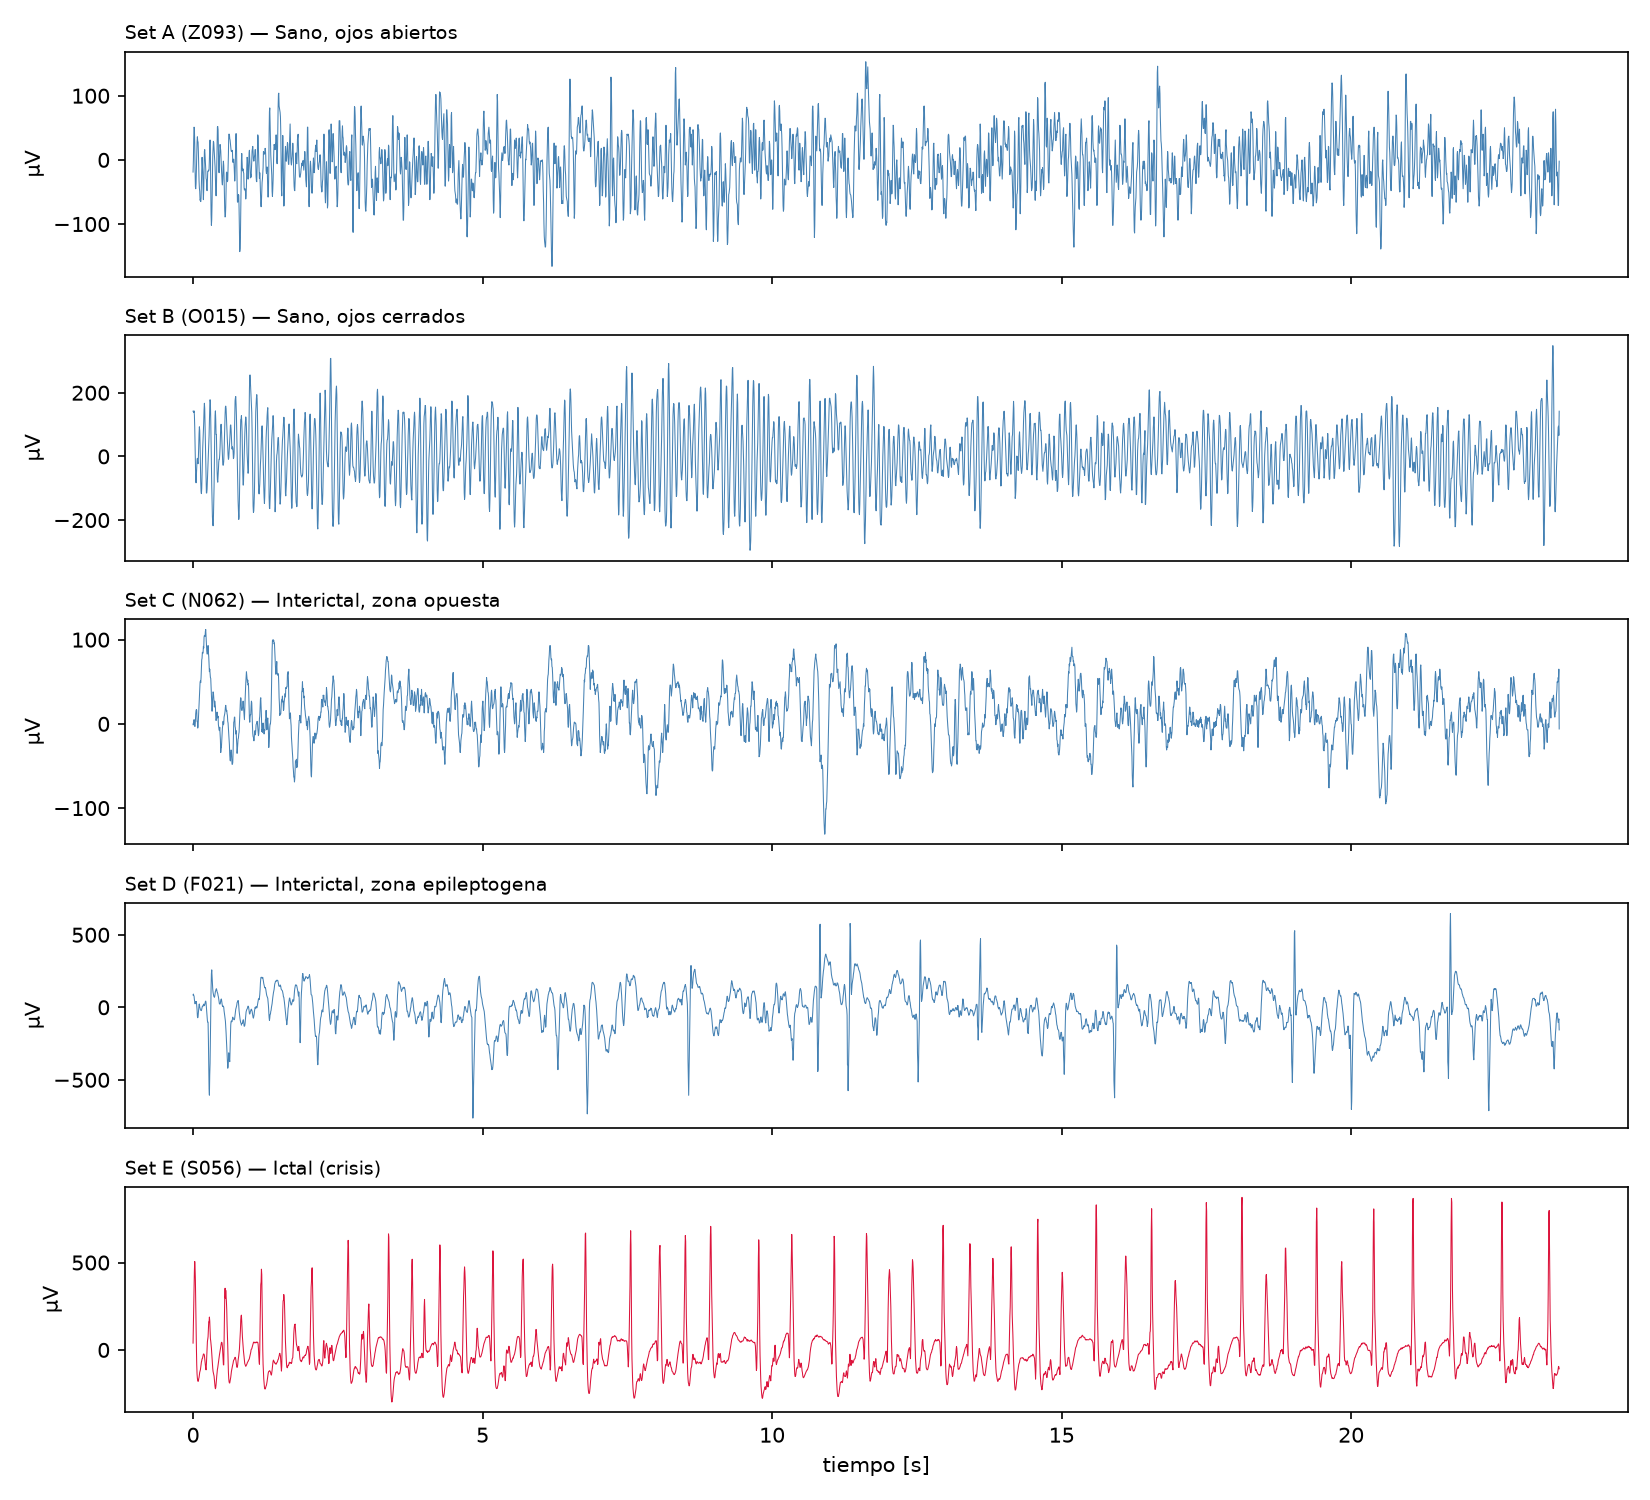
\includegraphics[width=\textwidth]{etapa1/ejemplos_por_set.png}
  \caption{Un segmento de 23,6~s de cada set de Bonn, en microvoltios. En rojo, el segmento ictal S056, el mismo del
           espectrograma de la Figura~\ref{fig:espectrograma_bonn}.}
  \label{fig:bonn_ejemplos}
\end{figure}

\subsection{Controles de calidad}

\begin{itemize}
  \item \textbf{Amplitud.} El desvío estándar del set E es 341~µV; el de los demás está entre 48 (A) y
        90~µV (D). La diferencia de amplitud, por sí sola, ya separa bastante las crisis (Capítulo~\ref{cap:fenomeno}).
  \item \textbf{Saturación.} El conversor de 12 bits satura en $\pm 2047$. Tres segmentos alcanzan ese valor:
        F009 (52 muestras) y S059 y S065 (20 muestras entre ambos). Son pocas muestras y se conservan.
  \item \textbf{Contenido por encima de 40 Hz.} Las series descargables no tienen aplicado el pasabajos de
        40~Hz del artículo original. La energía por encima de 40~Hz es como máximo el 0,39~\% del total (set A),
        así que aplicar el filtro casi no cambia las señales.
\end{itemize}

\subsection{Limitación}

La base no dice a qué paciente pertenece cada segmento. Al hacer validación cruzada, segmentos del mismo
paciente pueden quedar a la vez en entrenamiento y en prueba, de modo que las métricas sobrestiman lo que
pasaría con un paciente nuevo. Además, los segmentos se eligieron sin artefactos y cada clase viene de
condiciones de registro distintas (superficie contra intracraneal), lo que facilita la separación. Bonn sirve
para estudiar el fenómeno, no para medir el desempeño clínico; eso se hace con CHB-MIT.

\section{Base CHB-MIT}
\label{sec:chbmit}

\subsection{Descripción}

La base CHB-MIT \parencite{shoeb2009,guttag2010}, distribuida por PhysioNet \parencite{goldberger2000} con
licencia ODC-By~1.0, tiene registros de EEG de superficie de pacientes pediátricos del Children's Hospital
Boston, tomados durante varios días después de suspender la medicación para registrar crisis antes de una
posible cirugía. Las señales están muestreadas a 256~Hz con 16 bits, en el sistema internacional 10-20 con
montaje bipolar. El inicio y el fin de cada crisis fueron anotados por especialistas, con resolución de
1~s, en los archivos \texttt{chbNN-summary.txt}.

Se usan seis pacientes: chb01, chb02, chb03, chb05, chb08 y chb10, con 200 archivos EDF (8,8~GB). Todos
los archivos se verificaron contra las sumas SHA-256 publicadas por PhysioNet. La Tabla~\ref{tab:pacientes}
resume los datos.

\begin{table}[ht]
\centering
\caption{Pacientes de CHB-MIT usados. Ventanas de 4~s; ``borde'' son las que tocan una crisis solo en parte.}
\label{tab:pacientes}
\begin{tabular}{lcrrrrrrr}
\toprule
Paciente & Sexo, edad & Archivos & Horas & Ventanas & Ictales & Borde & Crisis & Duración [s] \\
\midrule
chb01 & F, 11  & 42 & 40,6 & 36\,496 & 107 & 8  & 7 & 27--101 \\
chb02 & M, 11  & 36 & 35,3 & 31\,739 & 41  & 4  & 3 & 9--82 \\
chb03 & F, 14  & 38 & 38,0 & 34\,201 & 96  & 10 & 7 & 47--69 \\
chb05 & F, 7   & 39 & 39,0 & 35\,102 & 136 & 7  & 5 & 96--120 \\
chb08 & M, 3,5 & 20 & 20,0 & 18\,005 & 226 & 8  & 5 & 134--264 \\
chb10 & M, 3   & 25 & 50,0 & 45\,020 & 105 & 12 & 7 & 35--89 \\
\midrule
Total &        & 200 & 222,8 & 200\,563 & 711 & 49 & 34 & \\
\bottomrule
\end{tabular}
\end{table}

Las 34 crisis suman 2940~s: el \textbf{0,366~\%} del tiempo registrado. Hay unas 280 ventanas sin crisis por
cada ventana ictal. Las crisis de chb08 son las más largas (hasta 264~s) y las de chb02, las más cortas (9~s).

\subsection{Canales}

Se usan los 18 canales del montaje bipolar ``doble banana'', comunes a todos los archivos de estos pacientes:
\begin{center}
\small
FP1-F7, F7-T7, T7-P7, P7-O1, FP1-F3, F3-C3, C3-P3, P3-O1, FP2-F4, F4-C4, C4-P4, P4-O2,\\
FP2-F8, F8-T8, T8-P8, P8-O2, FZ-CZ, CZ-PZ.
\end{center}
Los archivos tienen un canal 23 que repite T8-P8 y se descarta.

\section{Preprocesamiento de CHB-MIT}
\label{sec:preproc}

El script \texttt{scripts/preprocesar\_chbmit.py} procesa cada EDF una sola vez, en paralelo, y guarda un
archivo \texttt{.npz} por registro. Los pasos son:
\begin{enumerate}
  \item \textbf{Lectura} de los 18 canales con MNE y conversión a µV.
  \item \textbf{Filtrado} pasabanda Butterworth de orden 4 entre 0,5 y 40~Hz, de fase cero
        (\texttt{sosfiltfilt}), sobre el registro completo para evitar efectos de borde en cada ventana.
  \item \textbf{Ventanas} consecutivas, sin solapamiento, de $L = 4$~s (1024 muestras).
  \item \textbf{Espectrograma} de cada ventana y canal: Hann de 256 muestras (1~s), salto de 128 (0,5~s), lo que
        da 7 cuadros. Se guardan las frecuencias de 1 a 40~Hz (40 valores) en escala $\log_{10}$: un tensor de
        $18\times40\times7$ por ventana, que es la entrada de la CNN.
  \item \textbf{Potencia por banda}: el promedio de los 7 cuadros es la PSD de Welch; se integra con la regla del
        trapecio en las 5 bandas clínicas (delta 0,5--4, theta 4--8, alfa 8--13, beta 13--30 y gamma 30--40~Hz) y
        se toma $\log_{10}$. Resultan 90 atributos por ventana, la entrada de los modelos convexos.
  \item \textbf{Etiquetas}: para la ventana $w = [t_0, t_0 + L)$ y las crisis anotadas $[a_j, b_j]$,
        \begin{equation}
          y(w) =
          \begin{cases}
            1 \ \text{(ictal)} & \text{si } a_j \le t_0 \text{ y } t_0 + L \le b_j \text{ para algún } j, \\
            \text{borde} & \text{si la ventana se superpone con una crisis pero no está contenida}, \\
            0 \ \text{(sin crisis)} & \text{en otro caso.}
          \end{cases}
        \end{equation}
  \item \textbf{Amplitud máxima} de cada ventana, para analizar artefactos.
\end{enumerate}
Resultan 200\,563 ventanas: 711 ictales, 49 de borde y 199\,803 sin crisis.

Las ventanas de borde mezclan los dos estados, y la anotación tiene unos segundos de incertidumbre, así que no se
usan para entrenar. No se descartan ventanas por artefactos: un detector real tiene que funcionar con ellos.

\section{Análisis exploratorio}
\label{sec:exploratorio}

\subsection{Una crisis en la señal}

La Figura~\ref{fig:chb01_cruda} muestra los 18 canales alrededor de la primera crisis de chb01 (archivo
chb01\_03, de 2996 a 3036~s). Antes de la crisis se ven ráfagas de 10--14~Hz en los canales frontales, que son
actividad normal. Al empezar la crisis aparece una descarga rítmica de gran amplitud en casi todos los canales.
Después del fin anotado queda actividad lenta de gran amplitud: es el estado \emph{post-ictal}, que se etiqueta
como ``sin crisis'' y es una fuente esperable de falsas alarmas.

\begin{figure}[ht]
  \centering
  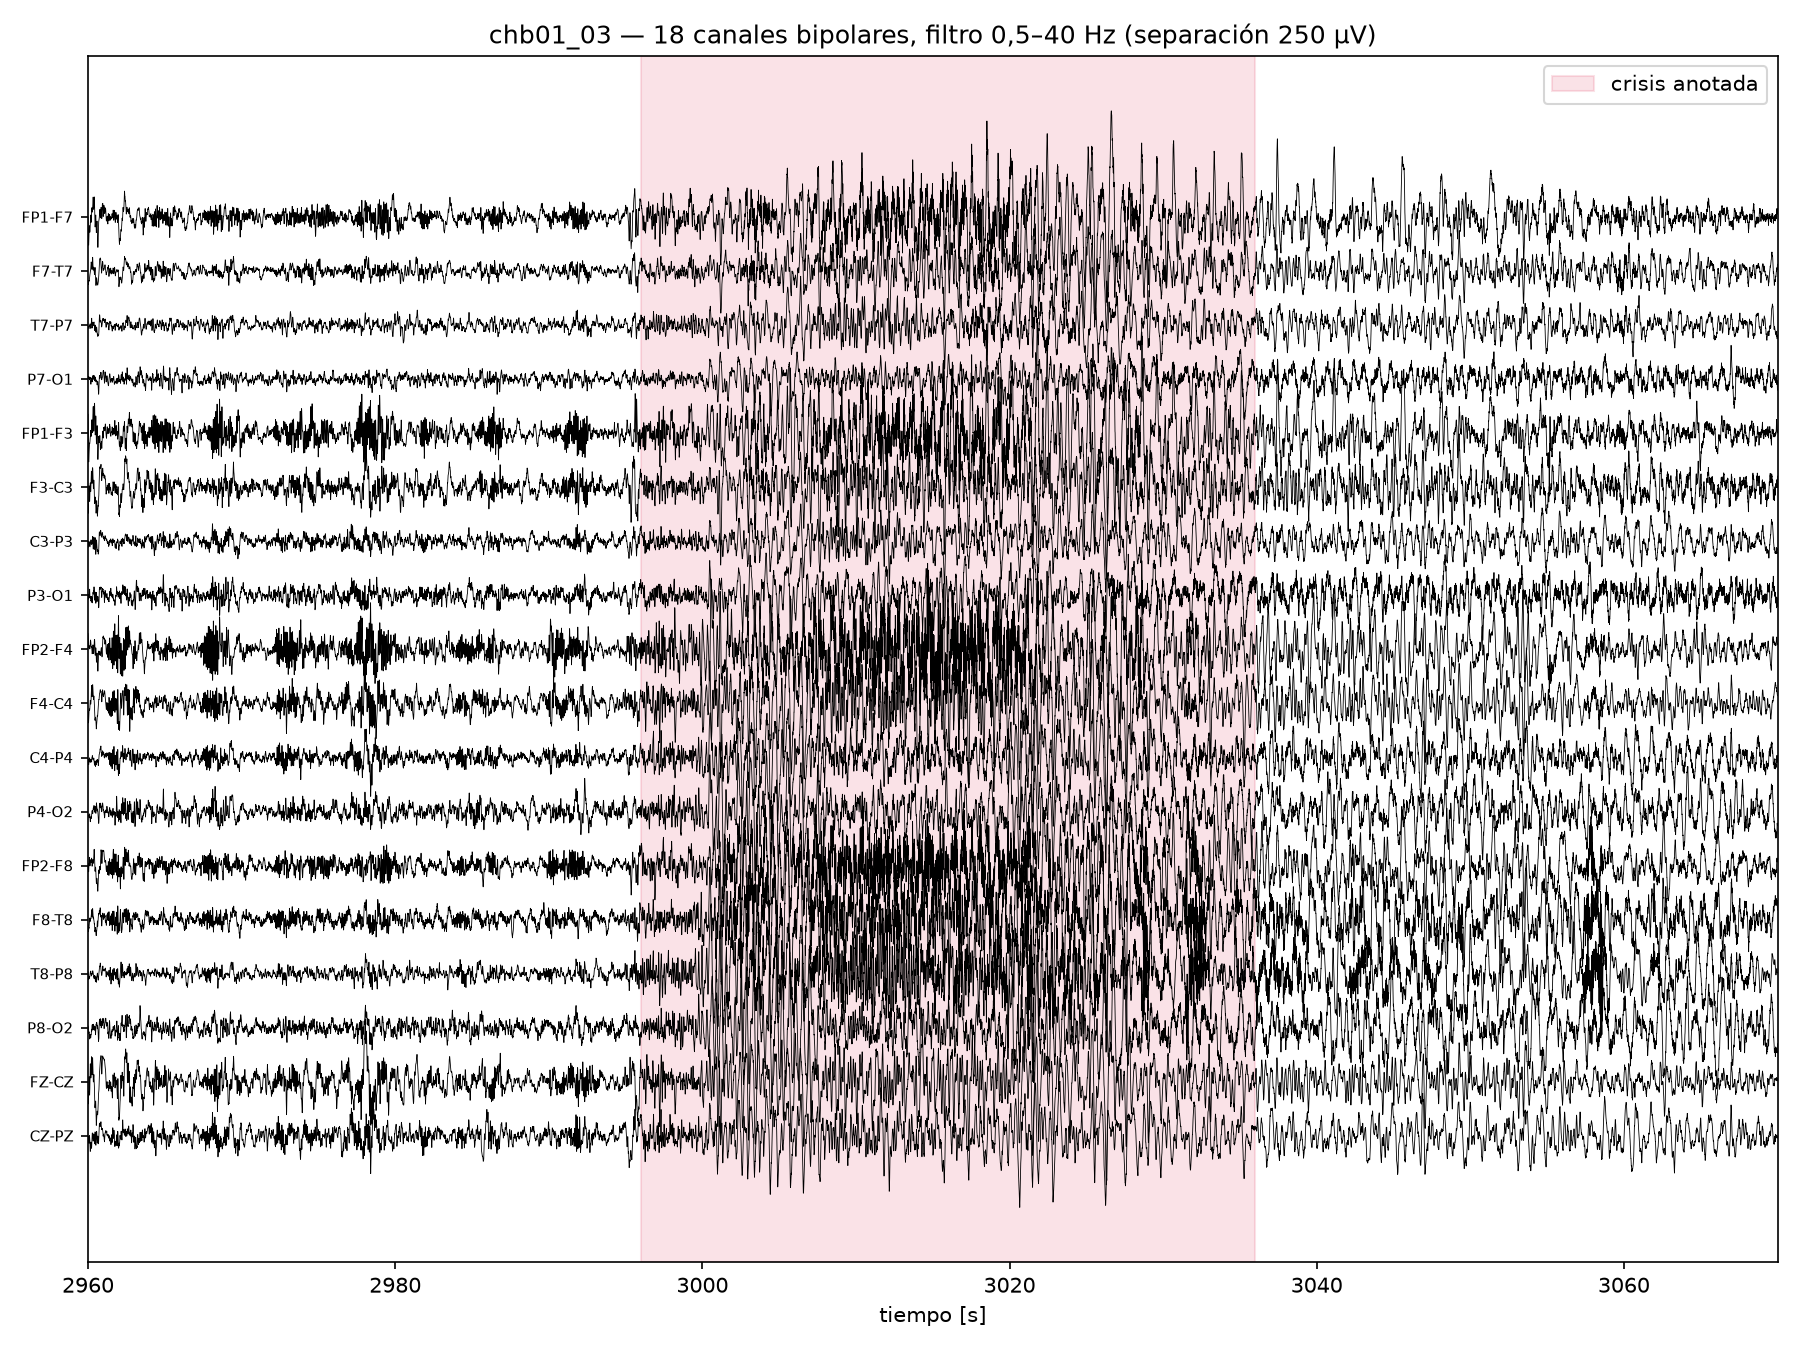
\includegraphics[width=\textwidth]{etapa2/chb01_03_crisis_cruda.png}
  \caption{Registro chb01\_03, 18 canales bipolares filtrados entre 0,5 y 40~Hz. La banda sombreada es la crisis
           anotada (2996--3036~s).}
  \label{fig:chb01_cruda}
\end{figure}

El espectrograma del canal con mayor amplitud durante la crisis (Figura~\ref{fig:chb01_espectrograma}) muestra
que la potencia sube en todo el rango de 1 a 40~Hz, sobre todo por debajo de 8~Hz, que es la descarga rítmica de
la ecuación~\eqref{eq:descarga}. Las líneas horizontales cerca de 16 y 32~Hz están presentes en todo el registro:
son interferencia de banda angosta del equipo, el término $\eta_c(t)$ del modelo~\eqref{eq:modelo_eeg}. Durante la
crisis quedan tapadas por la descarga.

\begin{figure}[ht]
  \centering
  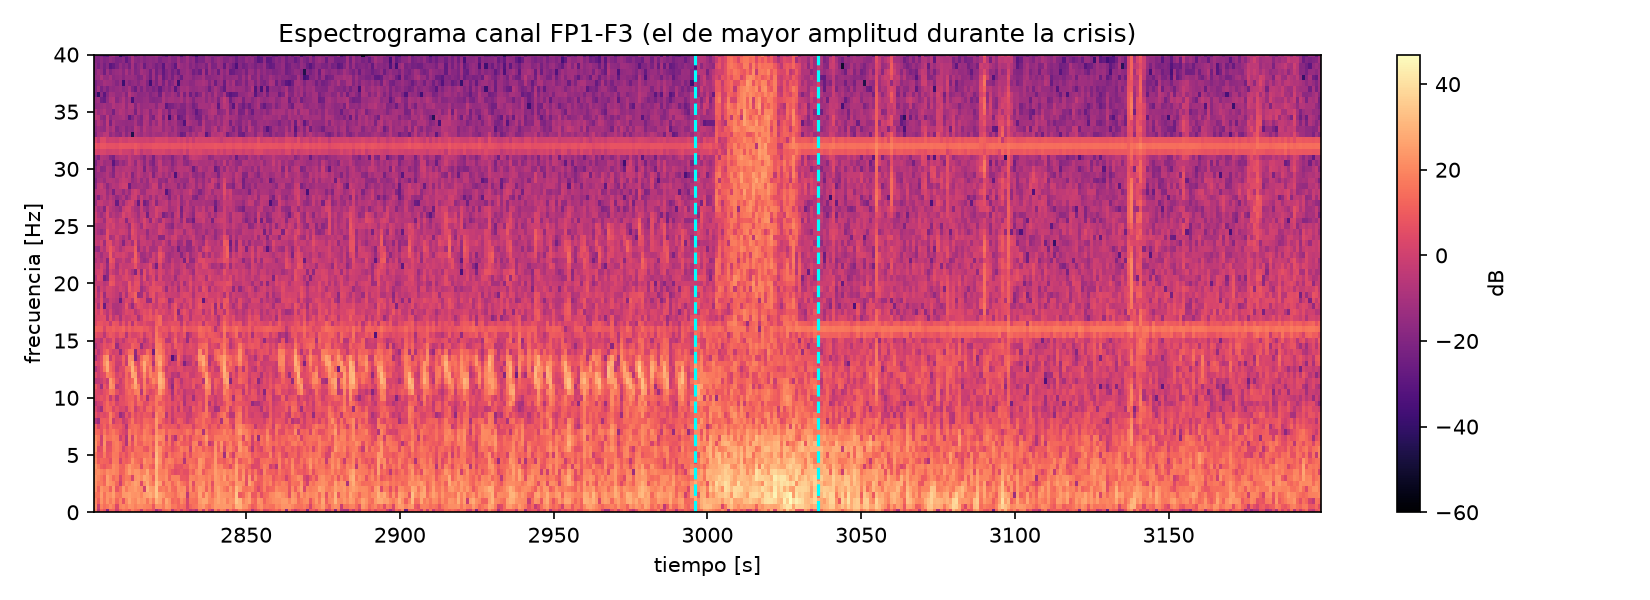
\includegraphics[width=\textwidth]{etapa2/chb01_03_espectrograma.png}
  \caption{Espectrograma (Hann de 2~s, 50~\% de solapamiento) alrededor de la crisis de chb01\_03. Las líneas
           punteadas marcan el inicio y el fin anotados.}
  \label{fig:chb01_espectrograma}
\end{figure}

\subsection{Potencia por banda y variabilidad entre pacientes}

La Figura~\ref{fig:bandas_pacientes} compara la potencia por banda (promedio de los 18 canales) en ventanas con y
sin crisis, para cada paciente, y la Tabla~\ref{tab:dif_log} resume la diferencia de las medias en escala
logarítmica.

\begin{figure}[ht]
  \centering
  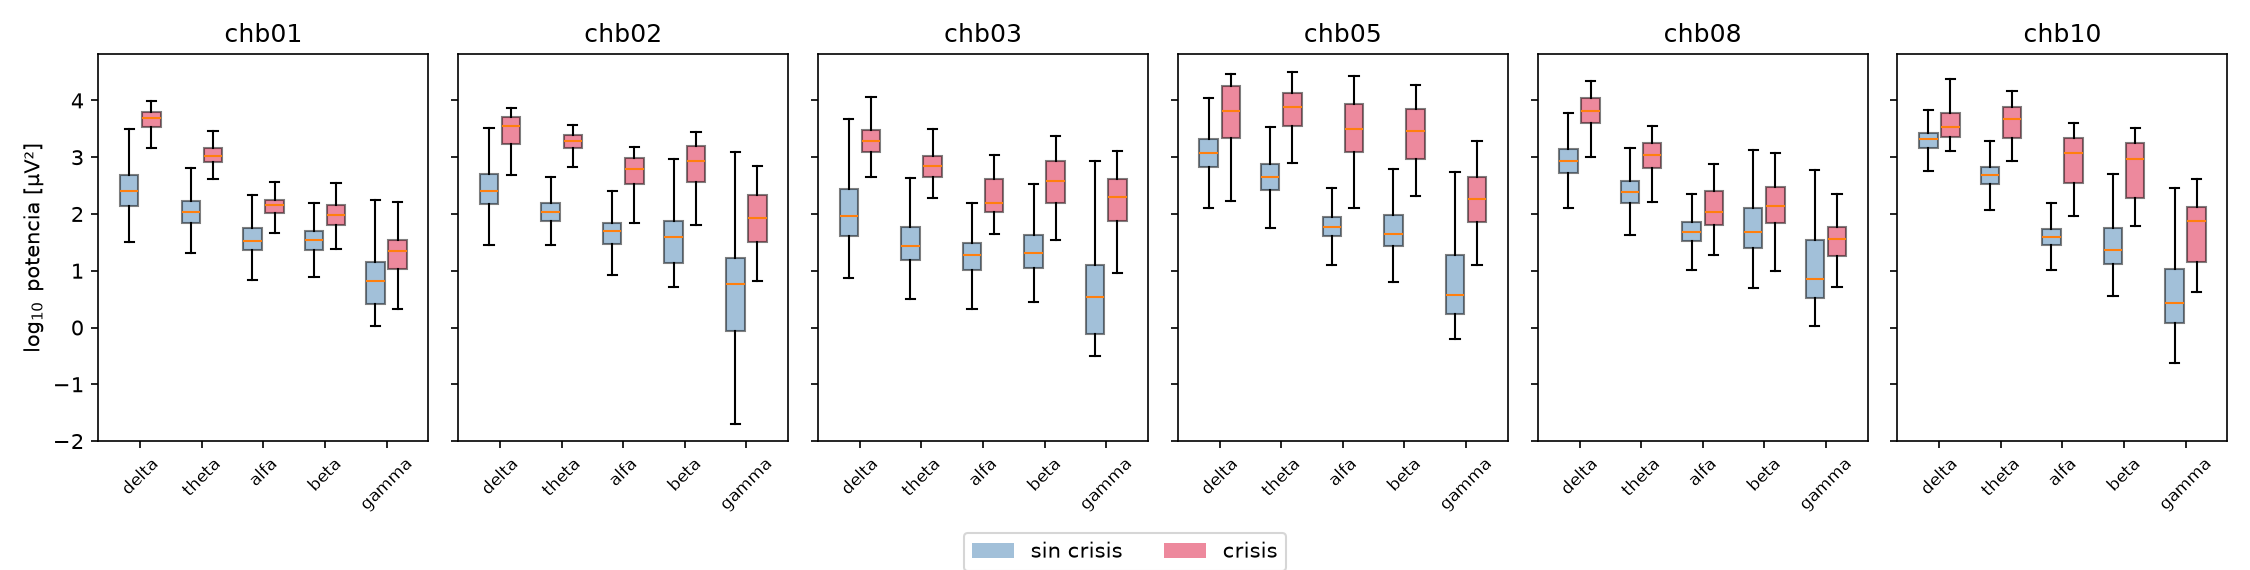
\includegraphics[width=\textwidth]{etapa2/potencia_bandas_por_paciente.png}
  \caption{$\log_{10}$ de la potencia por banda, promedio de los 18 canales, en ventanas sin crisis (azul) y con
           crisis (rojo), por paciente.}
  \label{fig:bandas_pacientes}
\end{figure}

\begin{table}[ht]
\centering
\caption{Diferencia media de $\log_{10}$ de la potencia entre ventanas con y sin crisis. Un valor de 1 equivale a
10 veces más potencia. En negrita, la banda de mayor aumento en cada paciente.}
\label{tab:dif_log}
\begin{tabular}{lrrrrr}
\toprule
Paciente & delta & theta & alfa & beta & gamma \\
\midrule
chb01 & \textbf{1,19} & 0,98 & 0,55 & 0,41 & 0,43 \\
chb02 & 0,99 & 1,19 & 1,05 & \textbf{1,25} & 1,24 \\
chb03 & 1,25 & 1,33 & 1,02 & 1,18 & \textbf{1,63} \\
chb05 & 0,68 & 1,20 & \textbf{1,69} & 1,67 & 1,47 \\
chb08 & \textbf{0,83} & 0,62 & 0,40 & 0,39 & 0,47 \\
chb10 & 0,34 & 0,91 & \textbf{1,33} & 1,29 & 1,07 \\
\bottomrule
\end{tabular}
\end{table}

Tres observaciones guían el resto del trabajo:
\begin{enumerate}
  \item \textbf{La potencia sube siempre.} En todos los pacientes y en todas las bandas, entre $10^{0{,}34} \approx 2$ y
        $10^{1{,}69} \approx 50$ veces. Es lo que predice el modelo aditivo (ecuación~\eqref{eq:dif_log}) y justifica usar la
        potencia por banda como atributo.
  \item \textbf{La banda que más sube depende del paciente.} Delta y theta en chb01 y chb08; alfa y beta en chb05 y
        chb10. Corresponde a frecuencias fundamentales $f_0$ distintas de la descarga. Un detector que sirva para
        pacientes nuevos tiene que combinar bandas.
  \item \textbf{El nivel basal también depende del paciente.} La potencia delta de chb10 \emph{sin} crisis (mediana
        $\approx 3{,}3$ en $\log_{10}$) está cerca de la de chb01 \emph{con} crisis ($\approx 3{,}7$). Un umbral fijo sobre una
        banda no sirve para todos. Es el término $2\log g_{p,c}$ del modelo, y motiva la calibración por paciente.
\end{enumerate}
chb08 es el paciente con menor aumento (0,4 a 0,8): sus crisis, largas y de menor amplitud relativa, son las más
difíciles de detectar.

\subsection{Artefactos de amplitud}

La mediana de la amplitud máxima por ventana sin crisis va de 178~µV (chb03) a 344~µV (chb08), y su percentil 99,
de 878 a 1430~µV. El percentil 99 de las ventanas sin crisis es del mismo orden que la mediana de las ventanas con
crisis (469 a 1252~µV): hay muchas ventanas normales con artefactos de amplitud comparable a una crisis, y la
amplitud sola no alcanza para detectar.

\section{Particiones}
\label{sec:particiones}

Las ventanas consecutivas de un registro están muy correlacionadas. Si se reparten al azar entre entrenamiento
y prueba, el modelo puede reconocer el registro y las métricas salen infladas (fuga de información). En CHB-MIT
todas las particiones son \emph{por paciente}.
\begin{itemize}
  \item \textbf{Bonn:} validación cruzada estratificada de 10 particiones, repetida 5 veces (con la limitación de la
        Sección~\ref{sec:bonn}).
  \item \textbf{CHB-MIT, LOPO:} 6 particiones, cada una deja afuera un paciente. Para los modelos convexos.
  \item \textbf{CHB-MIT, partición fija:} para la CNN y la comparativa de optimizadores, donde repetir 6 particiones
        con 6 optimizadores, 3 tasas y 5 semillas sería demasiado costoso sin GPU. Se eligió para que los tres
        conjuntos tengan una cantidad parecida de segundos de crisis (Tabla~\ref{tab:particion}).
\end{itemize}

\begin{table}[ht]
\centering
\caption{Partición fija por paciente de CHB-MIT.}
\label{tab:particion}
\begin{tabular}{llrrrr}
\toprule
Conjunto & Pacientes & Horas & Ventanas & Ictales & Crisis \\
\midrule
Entrenamiento & chb02, chb05, chb08 & 94,3 & 84\,846 & 403 & 13 \\
Validación    & chb01               & 40,6 & 36\,496 & 107 & 7 \\
Prueba        & chb03, chb10        & 88,0 & 79\,221 & 201 & 14 \\
\bottomrule
\end{tabular}
\end{table}

El conjunto de validación se usa para elegir la tasa de aprendizaje, la época de parada y el umbral de
Neyman-Pearson. El de prueba se evalúa una sola vez con el modelo elegido.

\section{Calibración por paciente}
\label{sec:calibracion}

Según el modelo~\eqref{eq:modelo_eeg}, el logaritmo de la potencia de cada canal y banda tiene un término
$2\log g_{p,c}$ que depende solo del paciente. Para eliminarlo, a cada atributo de cada paciente se le resta su
mediana sobre \emph{todas} las ventanas de ese paciente:
\begin{equation}
  \tilde x_{t,j} = x_{t,j} - \operatorname{mediana}_{u \in \text{paciente}(t)}\, x_{u,j}.
  \label{eq:calibracion}
\end{equation}
Se usa la mediana y no la media porque es robusta: las crisis son menos del 1~\% de las ventanas y casi no la
mueven, de modo que estima el nivel basal. La calibración \emph{no usa etiquetas}. En la práctica equivale a
registrar un rato al paciente nuevo antes de usar el detector, lo cual es razonable en una unidad de monitoreo,
donde los registros duran días.

La misma calibración se aplica al espectrograma de entrada de la CNN: a cada canal y frecuencia se le resta la
mediana del paciente.

Hay que notar que, en los pacientes de prueba, la mediana se calcula con todo su registro, incluido el futuro. Un
sistema en línea tendría que usar una mediana de las primeras horas o una ventana móvil; como la mediana es estable
(depende del nivel basal, no de las crisis), no se espera que el resultado cambie mucho, pero no se verificó.
